\section{Introducción}
\subsection{Tipos de variables}
\subsubsection{Discretas}
En matemáticas, la palabra discreto hace referencia a aquellos objetos que estan contenido en los numeros enteros (e.g. 1,2,-1,0,3). Lo más usual es solo usar el conjunto de los naturales, pero en algunas ocasiones es necesario usar los enteros negativos. En estadistica, este tipo de variable
\subsubsection{Continuas}
Las variables continuas usan los números reales para su representación.
\subsection{Diferencias en los usos de variables discretas o continuas}
La diferencia entre el uso de cada tipo de variable en estadistica esta concentrada en la definición de cada objeto matemático como lo es la esperanza, el promedio, la varianza, etc. Por ejemplo, La probabilidad es calculada de la siguiente manera:\\

\begin{minipage}{0.5\linewidth}
    \begin{center}
        \textbf{Variable discreta}
    \end{center}
    \begin{equation*}
        \bar{x}=\sum_{i=0}^N f(x_i)x_i
    \end{equation*}
\end{minipage}
\begin{minipage}{0.5\linewidth}
    \begin{center}
        \textbf{Variable continua}
    \end{center}
    \begin{equation*}
        \bar{x}=\int_a^b f(x)dx
    \end{equation*}
\end{minipage}\\

Al escribirlas de esta manera se logra visualizar la gran semejanza que tienen las expresiones de las variables discretas y continuas.

\section{Frecuencias}
La función de las frecuencias en la estadistica es representar de manera clara el comportamiento de la variable aleatoria por analizar, esto nos dara una idea de que distribución lograria representar mejor al objeto que quiero modelar. Como vamos a analizar frecuencias necesariamente tendremos que delimitar que rango contaremos o clasificaremos cada dato, esto va dependiendo que dan fino tengamos los datos. El estandar para definir cada intervalo es la siguiente:\\
Sea $\chi$ mi variable aleatoria y N la cantidad de datos, entonces:
\begin{enumerate}
    \item Calcular el número de clasificaciones (clases) $k$, la cual se calcula como la raiz de N.
          \begin{equation*}
              k=\sqrt{N}
          \end{equation*}
    \item Calcular la amplitud (rango) de los datos:
          \begin{equation*}
              R=max(\chi)-min(\chi)
          \end{equation*}
    \item Calcular la distancia entre cada clase:
          \begin{equation*}
              R_c = \frac{R}{k}
          \end{equation*}
\end{enumerate}
Supongamos que tenemos los siguientes datos:
\begin{table}[H]
    \centering
    \begin{tabular}{|cccccccccc|}
        \hline
        138 & 146 & 168 & 146 & 161 & 164 & 158 & 126 & 173 & 144 \\\hline
        145 & 150 & 140 & 138 & 142 & 135 & 132 & 147 & 176 & 165 \\\hline
        147 & 142 & 144 & 136 & 163 & 135 & 150 & 125 & 148 & 135 \\\hline
        119 & 153 & 156 & 149 & 152 & 154 & 140 & 145 & 157 & 128 \\\hline
    \end{tabular}
    \caption{Valores aleatorios}
    \label{table:valores_aleatorios_introduccion}
\end{table}
Siguiendo el estandar para calcular la tabla de frecuencias sobre los datos de la tabla \ref{table:valores_aleatorios_introduccion} se obtiene lo siguiente:\\

\begin{minipage}{0.25\linewidth}
    \begin{align*}
        R & =max(\chi)-min(\chi) \\
          & = 57                 \\
    \end{align*}
\end{minipage}
\begin{minipage}{0.25\linewidth}
    \begin{align*}
        N & =40 \\
    \end{align*}
\end{minipage}
\begin{minipage}{0.25\linewidth}
    \begin{align*}
        k & =\sqrt{N}    \\
          & =6.3245\dots \\
          & =7           \\
    \end{align*}
\end{minipage}
\begin{minipage}{0.25\linewidth}
    \begin{align*}
        R_c & = \frac{57}{7} \\
            & = 8            \\
            & =9             \\
    \end{align*}
\end{minipage}
Por lo tanto, las clases seran definidas por los siguientes intervalos:
\begin{table}[H]
    \centering
    \begin{tabular}{cc}
        \hline
        Límite inferior & Límite superior \\ \hline
        119             & 127             \\
        128             & 136             \\
        137             & 145             \\
        146             & 154             \\
        155             & 163             \\
        164             & 172             \\
        173             & 181             \\ \hline
    \end{tabular}
    \caption{Intervalo de las clases calculados a partir de los datos contenidos en la tabla \ref{table:valores_aleatorios_introduccion}. }
    \label{table:intervalo_de_clases_introduccion}
\end{table}
Realizando el conteo de cuantos datos estan contenidos en cada clase de la tabla \ref{table:intervalo_de_clases_introduccion} se obtiene la tabla \ref{table:histograma_de_clases_introduccion}:
\begin{table}[H]
    \centering
    \begin{tabular}{ccc}
        \hline
        Límite inferior & Límite superior & Frecuencia \\ \hline
        119             & 127             & 3          \\
        128             & 136             & 6          \\
        137             & 145             & 10         \\
        146             & 154             & 11         \\
        155             & 163             & 5          \\
        164             & 172             & 3          \\
        173             & 181             & 2          \\ \hline
    \end{tabular}
    \caption{frecuencias de los datos de la tabla \ref{table:valores_aleatorios_introduccion} con las clases de la tabla \ref{table:intervalo_de_clases_introduccion}.}
    \label{table:histograma_de_clases_introduccion}
\end{table}
Para realizar la gráfica de estas frecuencias existen varias maneras, ya sea definiendo un punto medio o estableciendo cada intevarlo. El histograma producido por la tabla \ref{table:histograma_de_clases_introduccion} es el siguiente:
\begin{figure}[H]
    \centering
    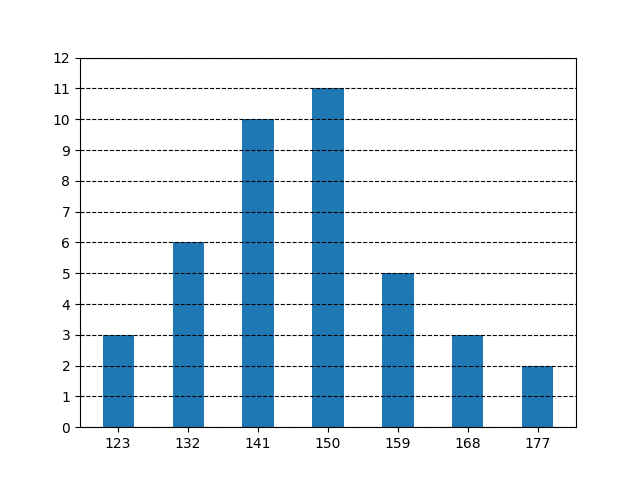
\includegraphics[scale=0.75]{Graphics/Histogram_1.png}
    \caption{Histograma obtenido a partir de los datos de la tabla \ref{table:valores_aleatorios_introduccion}}
\end{figure}